\documentclass{standalone}
\usepackage[x11names]{xcolor}
\usepackage{tikz}
\usetikzlibrary{shapes,arrows,decorations.markings, arrows.meta}
\usetikzlibrary {positioning}
\usetikzlibrary{calc}
\usetikzlibrary{patterns}
\usepackage{enumitem}
\usepackage{helvet}
\usepackage[T1]{fontenc}

%---------------------------------- Colors
\definecolor{color0}{RGB}{228,26,28}
\definecolor{color1}{RGB}{55,126,184}
\definecolor{color2}{RGB}{77,175,74}
\definecolor{color3}{RGB}{152,78,163}
\definecolor{color4}{RGB}{255,127,0}
\definecolor{color5}{RGB}{255,255,51}
\definecolor{color6}{RGB}{166,86,40}
\definecolor{color7}{RGB}{247,129,191}
\definecolor{color8}{RGB}{153,153,153}
\definecolor{color9}{RGB}{0,0,0}

\tikzstyle{item} = [rectangle, draw, fill=color0, text width=2cm, text centered, minimum height=2cm]

%----------------------------------------------------------------------------------
\def \nodeDistance {2.8cm}


\begin{document}
	\nopagecolor
	
	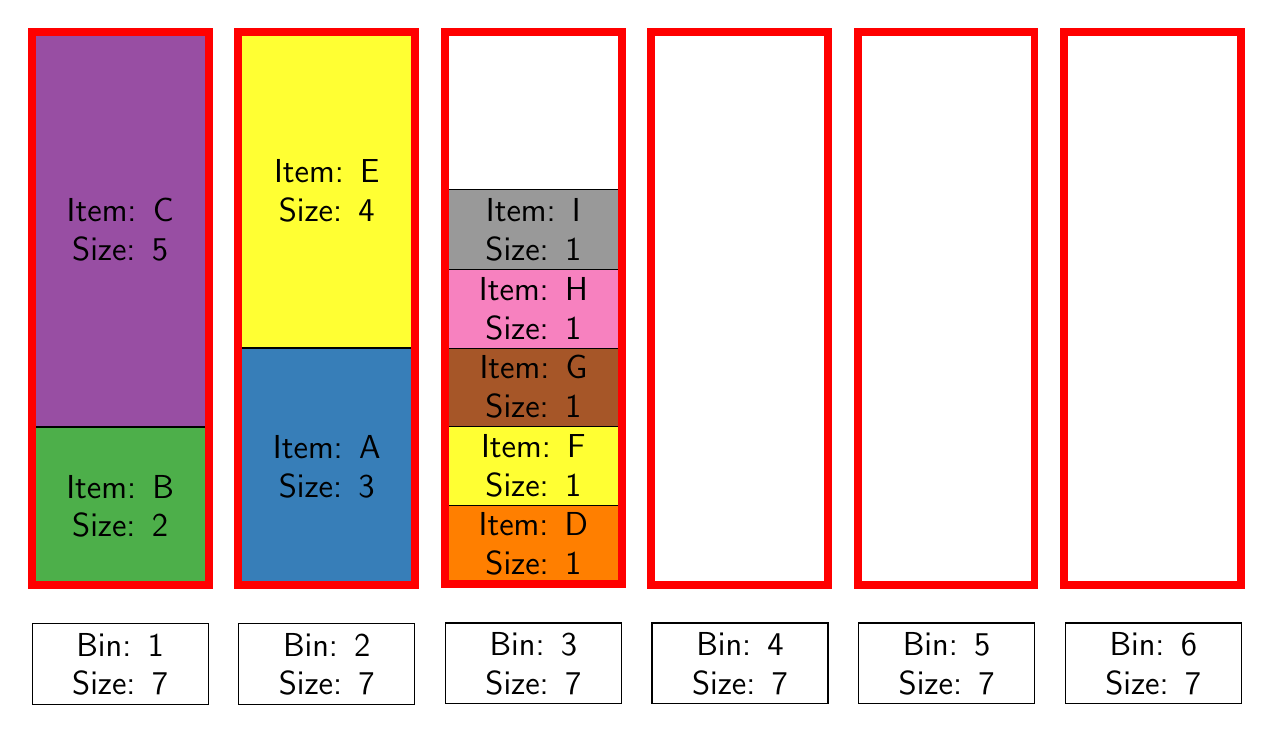
\begin{tikzpicture}[node distance = 2cm, auto,font=\sffamily\large]
		
	\node[item, minimum height=5cm, fill=color3](Item-C){Item: C\\Size: 5};
	\node[item, minimum height=2cm, fill=color2]at([yshift=-1cm]Item-C.south)(Item-B){Item: B\\Size: 2};
	
	\node[item, minimum height=3cm, fill=color1]at([xshift=1.5cm, yshift=0.5cm]Item-B.east)(Item-A){Item: A\\Size: 3};
	\node[item, minimum height=4cm, fill=color5]at([yshift=2cm]Item-A.north)(Item-E){Item: E\\Size: 4};

	
	\node[item, minimum height=1cm, fill=color4]at([xshift=1.5cm, yshift=-0.98cm]Item-A.east)(Item-D){Item: D\\Size: 1};
	
	
	\node[item, minimum height=1cm, fill=color5]at([yshift=0.48cm]Item-D.north)(Item-F){Item: F\\Size: 1};
	
	\node[item, minimum height=1cm, fill=color6]at([yshift=0.48cm]Item-F.north)(Item-G){Item: G\\Size: 1};
	
	\node[item, minimum height=1cm, fill=color7]at([yshift=0.48cm]Item-G.north)(Item-H){Item: H\\Size: 1};
	
	\node[item, minimum height=1cm, fill=color8]at([yshift=0.48cm]Item-H.north)(Item-I){Item: I\\Size: 1};
	
	\node[item, minimum height=1cm, fill=white] at([yshift=-1cm]Item-B.south)(Bin1){Bin: 1\\Size: 7};
	\node[item, minimum height=1cm, fill=white] at([yshift=-1cm]Item-A.south)(Bin2){Bin: 2\\Size: 7};
	\node[item, minimum height=1cm, fill=white] at([yshift=-1cm]Item-D.south)(Bin3){Bin: 3\\Size: 7};
	\node[item, minimum height=1cm, fill=white] at([xshift=1.5cm]Bin3.east)(Bin4){Bin: 4\\Size: 7};
	\node[item, minimum height=1cm, fill=white] at([xshift=1.5cm]Bin4.east)(Bin5){Bin: 5\\Size: 7};
	\node[item, minimum height=1cm, fill=white] at([xshift=1.5cm]Bin5.east)(Bin6){Bin: 6\\Size: 7};
	
	\draw[color=red,line width=1mm] (Item-B.south west) rectangle (Item-C.north east);
	\draw[color=red,line width=1mm] (Item-A.south west) rectangle (Item-E.north east);
	
	\node[circle,inner sep=0pt,minimum size=0pt](B3) at ([yshift=7.02cm]Item-D.south east) {};
	\draw[color=red,line width=1mm] (Item-D.south west) rectangle (B3);
	
	\node[circle,inner sep=0pt,minimum size=0pt](B4-1) at ([yshift=0.48cm]Bin4.north west) {};
	\node[circle,inner sep=0pt,minimum size=0pt](B4-2) at ([xshift=2.24cm, yshift=7.5cm]Bin4.north west) {};
	\draw[color=red,line width=1mm] (B4-1.south west) rectangle (B4-2);
	
		\node[circle,inner sep=0pt,minimum size=0pt](B5-1) at ([yshift=0.48cm]Bin5.north west) {};
	\node[circle,inner sep=0pt,minimum size=0pt](B5-2) at ([xshift=2.24cm, yshift=7.5cm]Bin5.north west) {};
	\draw[color=red,line width=1mm] (B5-1.south west) rectangle (B5-2);
	
		\node[circle,inner sep=0pt,minimum size=0pt](B6-1) at ([yshift=0.48cm]Bin6.north west) {};
	\node[circle,inner sep=0pt,minimum size=0pt](B6-2) at ([xshift=2.24cm, yshift=7.5cm]Bin6.north west) {};
	\draw[color=red,line width=1mm] (B6-1.south west) rectangle (B6-2);

	\end{tikzpicture}
\end{document}